\chapter{Impact of Neanderthal DNA on depression in Han Chinese individuals}
\section{Introduction} 
\textit{This chapter contains excerpts of a published paper Chiang et al. \cite{chiang2018comprehensive} presented here with permission from the authors.
}

To date, a range of strategies has been employed to characterize populations. In Genomes of the Netherlands (GoNL) (Francioli et al. 2014), the trio design allowed estimation of high-quality genotypes for both single nucleotide and structural variations with intermediate ($\sim13\times$) sequencing coverage and enabled the investigation of de novo mutations. In Sardinian (Sidore et al. 2015) and Icelandic (Gudbjartsson et al. 2015) population cohorts, extensive haplotype sharing within populations was used to inform accurate genotype calling among low- ($\sim4 – 6\times$) and intermediate- ($\sim20\times$) coverage sequencing of $\sim2,000 - 3,000$ individuals. In the UK10K project (Walter et al. 2015), low ($\sim7×\times$) whole-genome sequencing in 3,781 healthy samples from two British cohorts was combined with deep ($80\times$) exome sequencing in three disease cohorts to accurately detect low frequency and rare variants associated with quantitative traits. However, much like the genome-wide association studies preceding the current era of sequencing studies, most sequencing efforts are biased toward European populations. To address the need to comprehensively characterize non-European populations, we describe a resource of genetic variants in the world’s largest ethnic group, Han Chinese.

The whole-genome sequencing data set of the Han Chinese analyzed here adopted a different approach. We analyzed genetic variants from very low-coverage whole-genome sequencing data of 11,670 Han Chinese women, previously generated to study major depressive disorder (MDD) \cite{cai2015sparse}. With a median coverage of $1.7\times$, this data set is predicted to identify rare ($<0.5\%$) single nucleotide polymorphisms (SNPs) with high confidence (Li, Sidore, et al. 2011) and obtain accurate estimates of allele frequencies in a large sample. 

Previous analyses of the locations of Neanderthal segments within the genomes of non-African individuals indicated that some of the Neanderthal variants were adaptively beneficial while the bulk of Neanderthal variants were deleterious in the modern human genetic background \cite{harris2016genetic}, \cite{juric2016strength}. Specifically, a recent examination of Neanderthal-informative markers (NIMs) among large cohort of Europeans showed that these markers explained some proportions of the phenotypic risk of a number of diseases in the electronic health record \cite{simonti2016phenotypic}, including MDD. We sought to replicate this finding in East Asians as our data set was originally ascertained as a case–control study of MDD in Han Chinese women. \cite{cai2015sparse}.
\section{Results}
A total of 11,670 Han Chinese women were previously sequenced at a median coverage of $1.7\times$ per individual, of which 10,640 individuals and 25,057,223 SNPs remained after quality control (QC) (Cai et al. 2015,, 2017). Despite the low median coverage genome-wide, individual level genotype calls showed high concordance $(>96–97\%)$ in validation experiments (Cai et al. 2017). Furthermore, the allele frequencies in this data set are highly correlated (mean $r=0.995$ across chromosomes) to those from the East Asian sample in Exome Aggregation Consortium (ExAC; Lek et al. 2016). This observation suggests that any batch effect due to genotype calling in very low-coverage sequencing should not impact allele frequency estimates and their use in downstream analyses.
Restricting analysis to variants with minor allele counts (MAC) $\ge10$ (9,888,655 variants), we found that the alternate alleles of 477,792 (4.8\%), 567,731 (5.7\%), and 868,251 (8.8\%) variants are not seen in 1KG (phase 3), 1KG East Asians, and 1KG CHB+CHS panels, respectively (Table \ref{table:2.3}). We defined three minor allele frequency (MAF) categories: Common ($MAF \ge 0.05$), low frequency ($0.005\le MAF < 0.05$), and rare ($MAF < 0.005$). As expected, a large proportion (66-79\%) of novel alleles are rare in the population, and an additional 11-17\% of them are of low frequency (supplementary table S1, Supplementary Material online). We also identified $\sim82,000$ variants with $MAF \ge 0.05$ in our data set that are not seen in the 1KG CHB+CHS populations. Even though this class of variants is likely enriched for sequencing errors, a subset of these variants were identified in limited number of East Asians included in other recent large-scale sequencing efforts (Lek et al. 2016) and the frequency estimates are highly concordant (r=0.78 and 0.90 when compared with ExAC and GNOMAD databases, Fig \ref{fig:2.2}). Taken together, these observations suggest that our data set currently consists of the largest variant map in Han Chinese both in terms of span of the genome and in sample size.
\subsection{Genetic Relationship with Archaic Hominin Individuals}
Past studies of Neanderthal genomes have shown that the East Asians have inherited $\sim20\%$ more Neanderthal ancestry than Europeans and that this excess ancestry may reflect a second pulse of admixture in East Asians or a dilution of Neanderthal admixture in Europeans \cite{prfer2014complete},\cite{sankararaman2014genomic},\cite{vernot2014resurrecting},\cite{kim2015selection}. We largely recapitulated the relationship of a number of Neanderthal samples and Denisovan to the Han Chinese as previously reported (supplementary fig. S9, Supplementary Material online). We observed subtle differences in allele-sharing pattern and estimated Neanderthal ancestry $\sim(1.8–2\%)$ across China, though the difference is not significant after correcting for multiple testing (Fig \ref{fig:2.1}).
\section{Methods}
We extracted 75,539 SNPs that were previously identified to tag Neanderthal haplotypes in East Asian individuals in the 1KG project \cite{sankararaman2014genomic}, and assessed the contribution of these NIMs to depression in our cohort consisting 5,224 cases of MDD and 5,218 controls. The allele frequencies of these NIMs are highly correlated $(r=0.951)$ between our cohort and 1KG, suggesting that the NIMs are not overt outliers from the rest of the variants in our data set in terms of data quality. We tested the association between the NIMs and depression by performing a logistic regression of depression, controlling for age and the first ten PCs, for MDD and Melancholia. Using the current sample size and sequence data, we found no association surviving the Bonferroni correction (Fig \ref{fig:2.1}) and the QQ plots did not reveal any systematic inflation nor significant enrichment among top associated SNPs (data were not shown).

We also calculated the proportion of phenotypic variance explained by these NIMs using GCTA (Yang et al. 2011) for MDD. We used a prevalence of 7.5\% to transform the heritability to the liability scale. We found that the variance explained by the NIMs is $\sim1\%$, which is different from that reported in Simonti et al. $(\sim2\%)$ and is not significantly different from 0 $(P=0.12)$. Repeating the analysis with NIMs with MAF >0.01 as well as with no covariates did not qualitatively alter the results (Tables \ref{table:2.1}, \ref{table:2.2}). Finally, we found that the heritability explained by NIMs is not significantly different from that of a background set of SNPs chosen at random to match the NIMs by derived allele frequency decile and by Linkage Disequilibrium (LD) scores $(P>0.4)$. Our analysis may be under-powered given the smaller sample size and low coverage, but the results could suggest that the impact of Neanderthal ancestry on MDD differs between European and Han Chinese. Future investigation in larger cohorts will be informative.
%***********PBC***************
\section{Discussion}
A major limitation to our study is the reliance on allele frequency-based methods for analysis, as the very low-coverage data obscured the haplotypic patterns at the individual level and precluded direct merging and comparison to other reference data sets. Haplotype-based analysis may reveal additional structure beyond the two geographical axes found here. Nevertheless, our analysis framework relying heavily on allele frequency estimates is applicable to future very large-scale (>100,000 individuals) whole-genome sequencing studies, which in the short term will inevitably focus on ultra-low sequencing data such as those obtained through noninvasive prenatal testing. Despite these ongoing challenges to develop and employ appropriate analysis methods, our results collectively demonstrate the existence of significant variations in demographic and adaptive histories across Han Chinese populations. We demonstrated how the impact due to Neandertal ancestry on one type of trait, MDD and Melancholia, appears to differ between Han Chinese and Europeans. In general, these unique histories undoubtedly contributed to the variation of phenotype within Han Chinese as well as between Han Chinese and other global populations. Therefore, a better understanding of Han Chinese history will help in conducting and interpreting future medical genetic studies within the largest ethnic group of mankind.
\newpage
\section{Figures}
\begin{figure}[!htb]
    \centering
    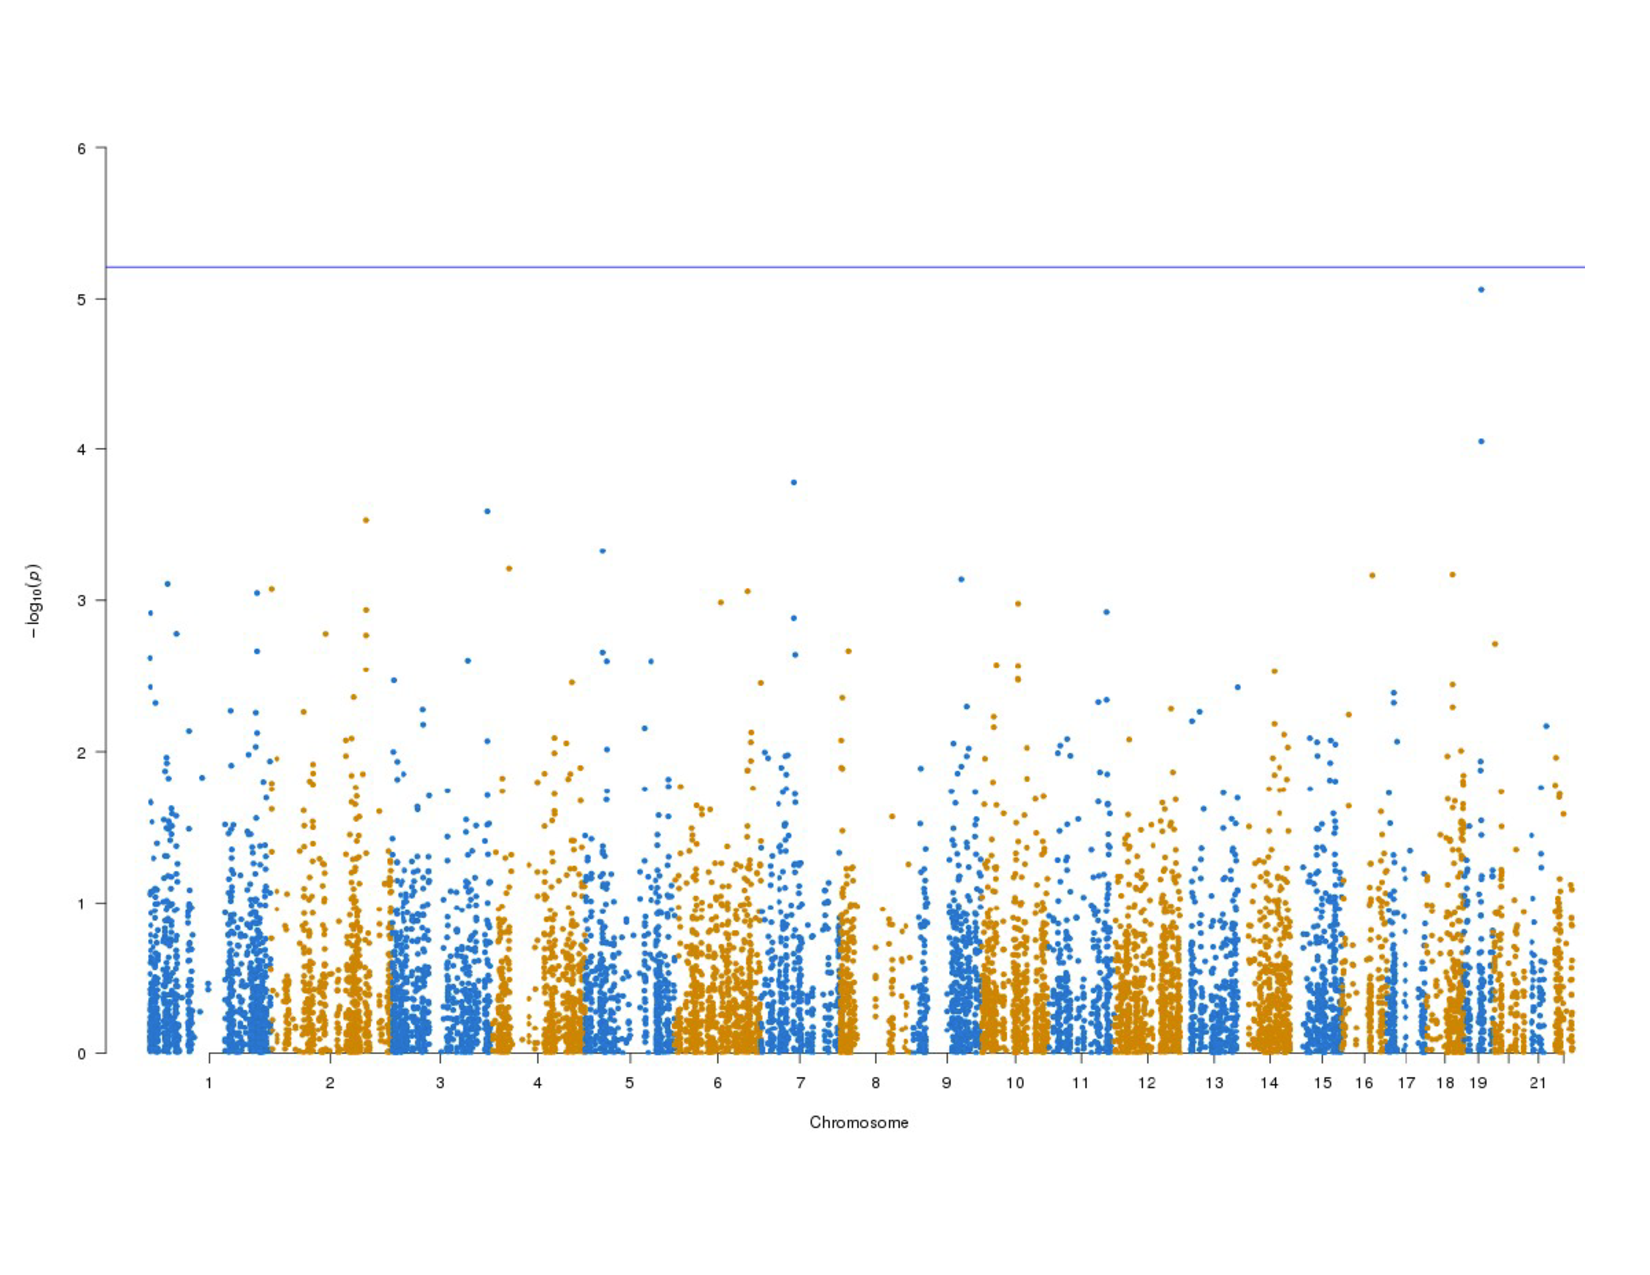
\includegraphics[width=\textwidth]{chapter2/figures/fig2.1.pdf}
    \caption{Manhattan plot for association of Neandertal-informative markers (NIMs) and MDD. We find no NIMs significantly associate with MDD. The blue line represents the Bonferroni correction threshold.}
    \label{fig:2.1}
\end{figure}
\clearpage


\begin{center}
  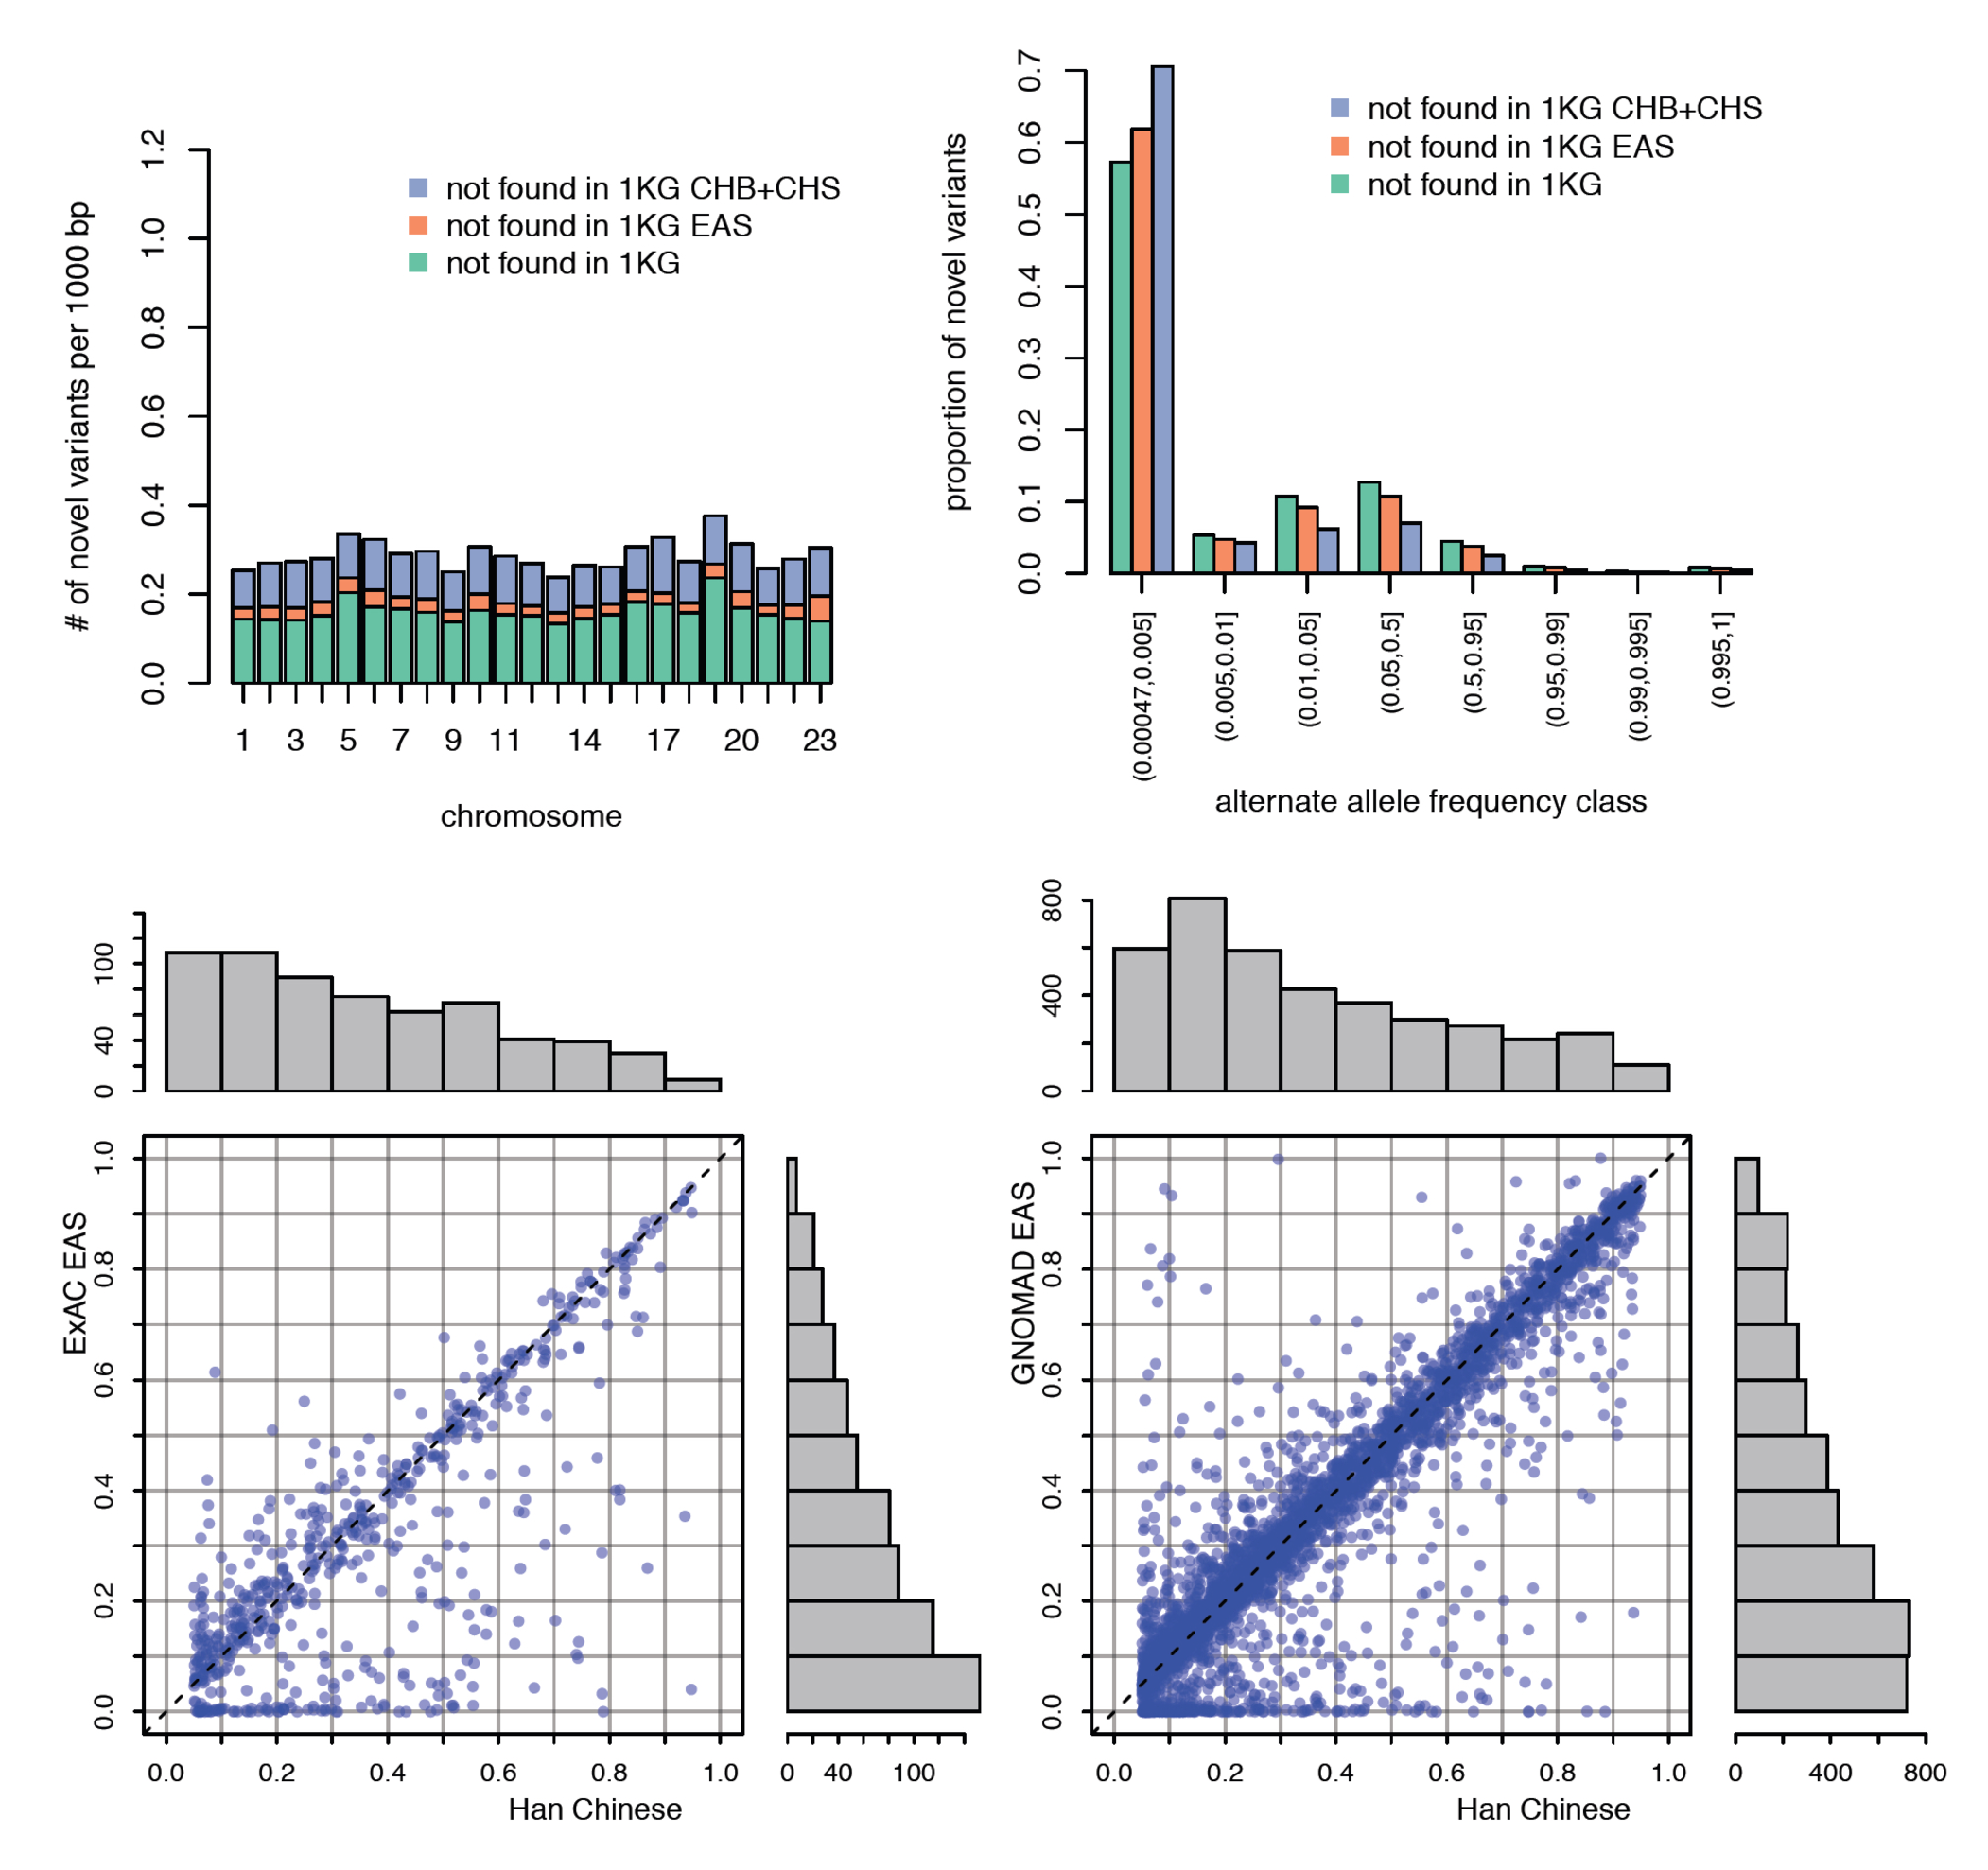
\includegraphics[ width=\textwidth]{chapter2/figures/fig2.2.pdf}
  \emph{Figure 2.2 (Caption on next page.)}
  \end{center}
  
\begin{figure}[!htb]
    \centering
    \caption{variant density, frequency spectra, and allele frequency comparisons for novel variants. We defined novel variants with respect to three increasing level of inclusiveness: those
with called alternative alleles that are not found among 1KG (phase3) CHB+CHS populations, 1KG
EAS super-population, and all 1KG populations. Note that if the alternative allele identified in our
dataset represents a previously unobserved allele in 1KG, it is considered a novel variant, even if the
site is otherwise variable in 1KG. (Top Left) Density of novel alleles discovered per 1000 bp, per
chromosome. Chromosome 23 signifies the X chromosome. (Top Right) Distribution of alternate
allele frequency of the novel alleles. For each novel allele that was common ($MAF \ge 0.05$) in our
dataset, we compared its frequency to that estimated from ExAC (Bottom Left) and GNOMAD (Bottom Right) if the same allele passed quality control filters and was called in at least 2,000 (out of
8,654) or 800 (out of 1,622) East Asian chromosomes in ExAC and GNOMAD, respectively. In total,
out of 82,626 common novel alleles not found in 1KG CHB+CHS, frequency comparisons were made for 644 alleles in ExAC and 40,544 alleles in GNOMAD (random 10\% of these alleles are shown here). The correlations were 0.78 and 0.90, respectively.}
    \label{fig:2.2}
\end{figure}


\FloatBarrier
\clearpage
\section{Tables}
\begin{longtable}[]{@{}llll@{}}
\toprule
\endhead
& $H^2_{NIM}$ & Standard error & p-value\tabularnewline
\bottomrule
All NIM & 0.009455 & 0.008175 & 0.1177\tabularnewline
$MAF \ge 0.01$ & 0.008081 & 0.007664 & 0.1386\tabularnewline
$MAF\ge 0.01$, no covariates & 0.013443 & 0.007650 & 0.0295\tabularnewline
\bottomrule
\caption{Heritability associated with Neanderthal-informative mutations
(NIMs) for MDD}
\label{table:2.1}
\end{longtable}

\begin{longtable}[]{@{}llll@{}}
\toprule
\endhead
& $H^2_{NIM}$& Standard error & p-value\tabularnewline
\bottomrule
All NIM & 0.010055 & 0.008867 & 0.1223\tabularnewline
$MAF \ge 0.01$ & 0.006631 & 0.008247 &
0.2051\tabularnewline
$MAF \ge 0.01$, no covariates & 0.010721 & 0.008249 & 0.086\tabularnewline
\bottomrule
\caption{Heritability associated with Neanderthal-informative mutations (NIMs) for Melancholia.}
\label{table:2.2}
\end{longtable}

\begin{table}[!ht]
    \centering
    \begin{tabular}{|l|l|l|l|l|l|l|l|}
    \hline
        Chr & \shortstack{FREQ\\ (0,\\\ 0.005]} & \shortstack{FREQ\\ (0.005,\\ 0.05]} & \shortstack{FREQ\\ (0.05,\\ 0.5]}  & \shortstack{MAC\\  $\ge 10$} & \shortstack{Novel\\ 1KG}& \shortstack{Novel\\ EAS} & 
        \shortstack{Novel\\ CHB+\\ CHS}\\ \hline
        1 & 1,343,061 & 163,396 & 400,089 & 746,698 & 35,854 & 42,022 & 63,290 \\ \hline
        2 & 1,489,539 & 170,075 & 420,949 & 793,269 & 34,855 & 41,666 & 65,670 \\ \hline
        3 & 1,212,220 & 146,233 & 372,469 & 685,664 & 28,081 & 33,632 & 54,029 \\ \hline
        4 & 1,155,002 & 145,299 & 383,272 & 690,219 & 28,936 & 34,813 & 53,651 \\ \hline
        5 & 1,091,572 & 129,719 & 331,457 & 610,644 & 36,821 & 42,802 & 60,665 \\ \hline
        6 & 1,044,524 & 137,817 & 360,191 & 652,006 & 29,219 & 35,802 & 55,266 \\ \hline
        7 & 962,541 & 113,402 & 310,643 & 556,322 & 26,689 & 30,905 & 46,405 \\ \hline
        8 & 961,513 & 104,469 & 286,434 & 519,804 & 23,278 & 27,624 & 43,402 \\ \hline
        9 & 732,741 & 89,897 & 227,055 & 418,914 & 19,519 & 23,029 & 35,290 \\ \hline
        10 & 837,611 & 99,357 & 267,928 & 484,979 & 22,215 & 27,179 & 41,506 \\ \hline
        11 & 851,586 & 91,851 & 260,208 & 466,401 & 20,793 & 24,230 & 38,504 \\ \hline
        12 & 792,885 & 100,571 & 248,101 & 457,006 & 20,327 & 23,264 & 36,063 \\ \hline
        13 & 593,970 & 73,948 & 190,863 & 345,579 & 15,415 & 18,237 & 27,483 \\ \hline
        14 & 552,395 & 67,394 & 173,684 & 320,535 & 15,551 & 18,346 & 28,421 \\ \hline
        15 & 506,764 & 62,374 & 153,593 & 286,766 & 15,794 & 18,335 & 26,796 \\ \hline
        16 & 571,041 & 60,257 & 161,897 & 297,775 & 16,521 & 18,633 & 27,761 \\ \hline
        17 & 484,841 & 53,251 & 136,736 & 258,266 & 14,421 & 16,463 & 26,634 \\ \hline
        18 & 475,960 & 57,359 & 149,977 & 273,187 & 12,392 & 14,085 & 21,350 \\ \hline
         19 & 373,806 & 48,412 & 119,786 & 224,128 & 13,998 & 15,854 & 22,261 \\ \hline
        20 & 395,775 & 43,630 & 112,815 & 210,807 & 10,641 & 12,990 & 19,724 \\ \hline
        21 & 222,299 & 25,482 & 76,266 & 133,070 & 7,369 & 8,492 & 12,446 \\ \hline
        22 & 232,448 & 30,142 & 71,407 & 136,040 & 7,461 & 9,005 & 14,299 \\ \hline
        X & 720,083 & 69,725 & 153,166 & 320,576 & 21,642 & 30,323 & 47,335 \\ \hline
        Tot & 17,604,177 & 2,084,060 & 5,368,986 & 9,888,655 & 477,792 & 567,731 & 868,251 \\ \hline
    \end{tabular}
    \caption{summary of variants discovered per chromosome. Novel variants are the subset of variants with minor allele count $(MAC) \ge 10$ in the current study that are also monomorphic or not reported in 1KG (phase 3), 1KG EAS, or 1KG CHB+CHS populations.}
\label{table:2.3}
\end{table}
